\section{Background and Related Work}
\label{chap:background}

%===============================================================
\subsection{B-Representation (B-Rep) Fundamentals}
%===============================================================

The Boundary Representation (B-Rep) is a fundamental data structure in Computer-Aided Design (CAD) systems. B-Reps describe 3D solid objects by explicitly representing their boundary surfaces. This representation form enables precise geometric modeling and is widely used in industrial design, mechanical engineering, and manufacturing.
The key components of a B-Rep include faces, edges, and vertices, along with their topological relationships.

\par

\textbf{Key characteristics of B-Reps:}
\begin{itemize}
	\item \textbf{Explicit Surface Representation}: Surfaces are defined using parametric equations (e.g., Non-Uniform Rational Basis Splines)
	\item \textbf{Topological Consistency}: Maintains relationships between geometric elements
	\item \textbf{Industry Standard}: Widely supported by professional CAD software (Autodesk, Solidworks, FreeCAD)
	\item \textbf{High Precision}: Suitable for manufacturing and detailed design specifications
\end{itemize}

%===============================================================
\subsection{Generative Models for CAD}
%===============================================================

Recent advances in deep learning have enabled the development of neural models capable of generating CAD geometry. Two complementary approaches have emerged: diffusion-based and autoregressive methods, each with distinct advantages for direct B-Rep synthesis.

\par

\textbf{Generative modeling approaches:}
\begin{itemize}
	\item \textbf{Autoregressive Models}: Generate sequences token-by-token, capturing dependencies
	\item \textbf{Diffusion Models}: Iteratively refine from noise, offering excellent quality
	\item \textbf{VAE-based Methods}: Learning compressed latent representations
	\item \textbf{Hybrid Approaches}: Combining multiple techniques for optimal performance
\end{itemize}

%===============================================================
\subsubsection{BrepGen: Diffusion-Based Approach}
%===============================================================

\cite{Xu2024brepgen} introduces BrepGen, a diffusion-based model for direct B-Rep generation. The key innovation is a \textit{structured latent geometry} representation that encodes B-Reps as hierarchical trees with three levels: faces, edges, and vertices.

\begin{figure}[h!]
	\centering
	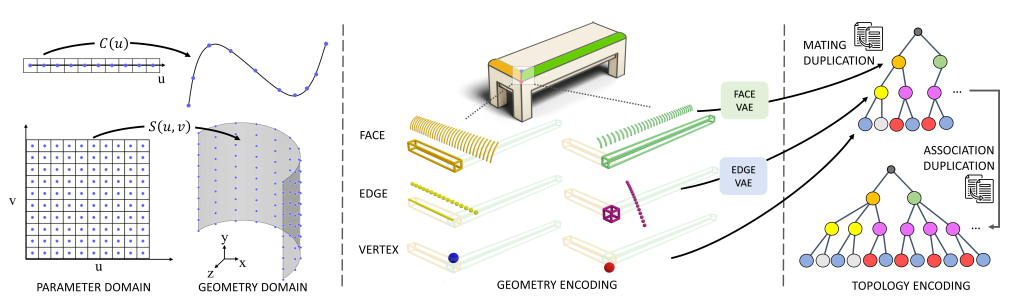
\includegraphics[width=1\textwidth]{figures/brepgen_encoding.png}
	\caption{Encoding B-rep's into point clouds: 32 x 32 points are sampled over each surface and 32 points over each edge of the solid. The faces and edges are then stored in a hierarchical tree which encodes the topology (connections between different faces and edges)}
	\label{fig:brepgen_encoding}
\end{figure}
\begin{figure}[h!]
	\centering
	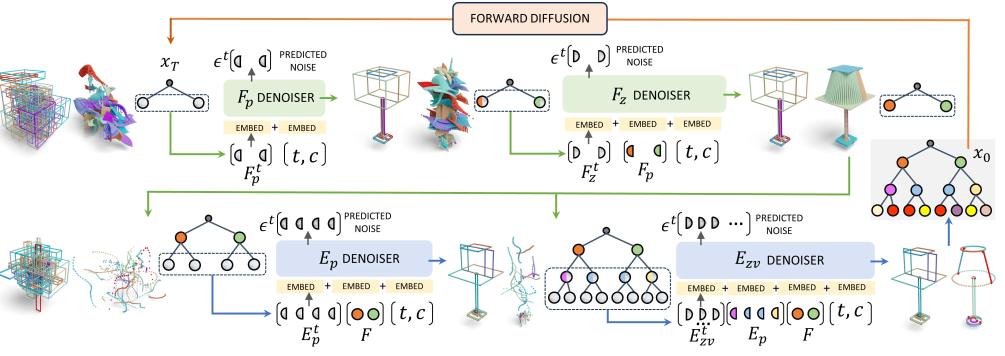
\includegraphics[width=1\textwidth]{figures/brepgen_model.png}
	\caption{Generating new B-rep's: The noise for faces and bounding boxes (spacial lmitis of the faces) is denoised with two denoisers. Conditioned on these faces, edge noise and bounding boxes are generated and again twice denoised}
	\label{fig:brepgen_model}
\end{figure}

 Postprocessing: The generated edge and and face pointclouds are sewed back into  B-rep's in .step format using the Open-Cascade library.



%===============================================================
\subsubsection{AutoBrep: Autoregressive Approach}
%===============================================================

\cite{Xu2025autobrep} presents AutoBrep, an autoregressive Transformer that unifies B-Rep geometry and topology into a single stream of discrete tokens. Unlike multi-stage diffusion, AutoBrep generates B-Reps end-to-end via next-token prediction Fig. \ref{fig:scheme}.

\begin{figure}[h!]
	\centering
	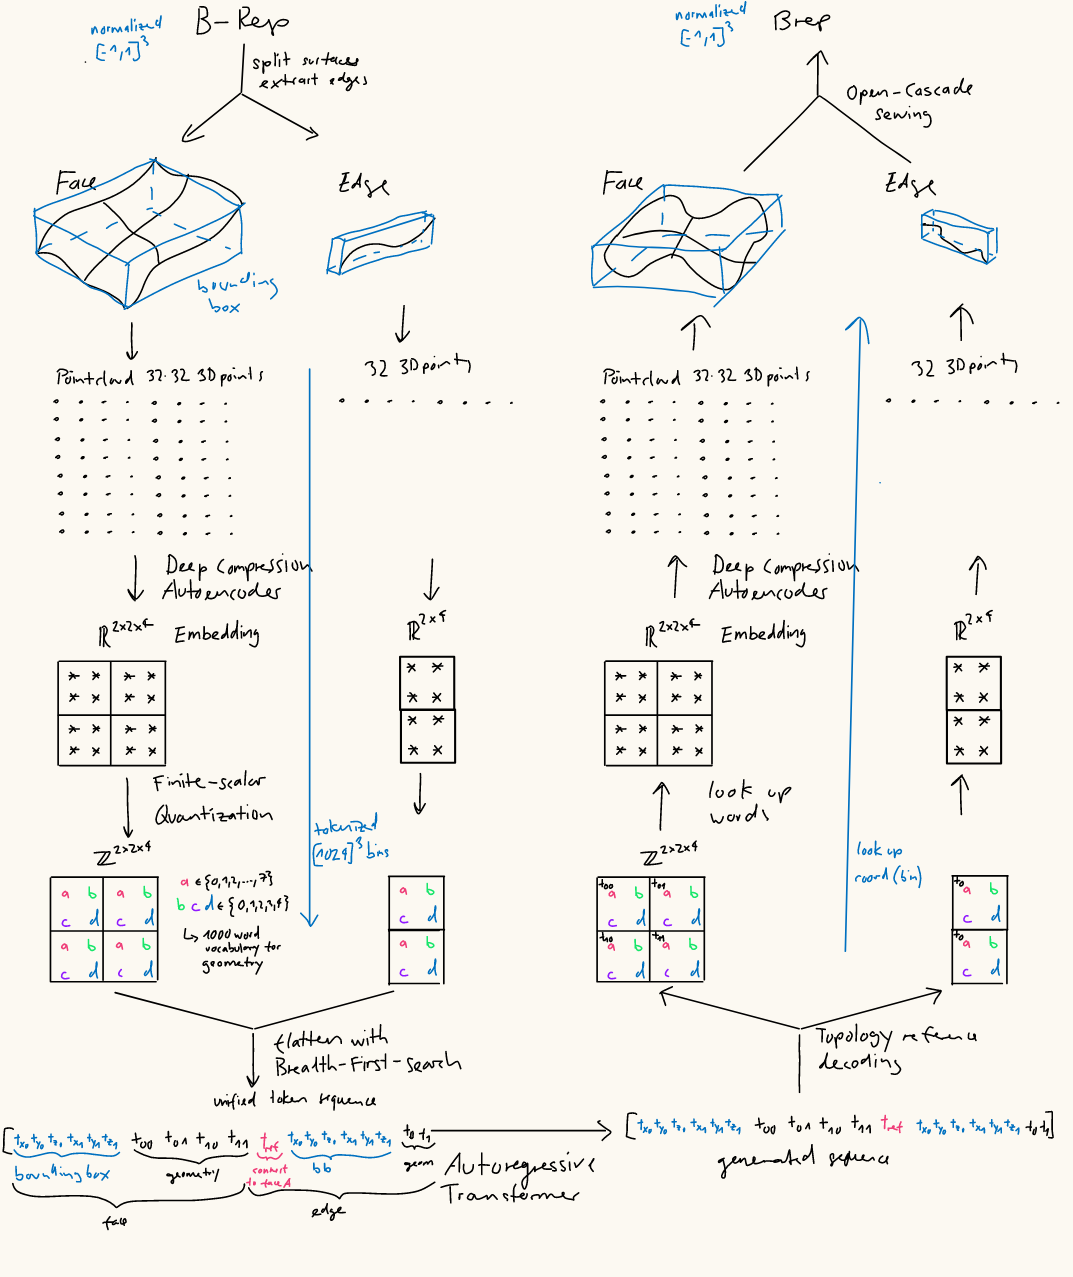
\includegraphics[width=1\textwidth]{figures/autobrep_scheme.png}
	\caption{Starting from the top left, the encoding into point clouds is equivalent to BrepGen. Next, the faces are encoded into Tokens using a VAE and quantized with finite scalar quantization into a 1000 word vocabulary. Tokens are then places in a sequence where the order is retrieved from a Breadth-First-Search over the surfaces and edges of the B-Rep. This sequence is then fed into a GPT-like transformer model using a causal mask. Then the transformer predicts the sequence (during training, else a new sequence) through next-token prediction and the process repeats in the opposite direction.}
	\label{fig:scheme}
\end{figure}

\par


Key advantages: (1) Single unified architecture vs. multi-stage pipeline, (2) 2--5$\times$ faster inference via next-token prediction, (3) Native support for B-Rep completion through next token prediction, (4) Scalability to 100+ face solids.

\par

\textbf{Comparison:}
\begin{itemize}
	\item \textbf{BrepGen}: Six modules (2 VAEs + 4 diffusion denoisers), multi-stage cascading, slower (~10 sec/sample), supports conditional generation
	\item \textbf{AutoBrep}: Three modules (2 autoencoders + 1 transformer), unified pipeline, faster (~0.46 sec/sample), natively supports autocompletion with face preservation
\end{itemize}

%===============================================================
\subsection{Low-Rank Adaptation (LoRA)}
%===============================================================

LoRA (Low-Rank Adaptation) is a parameter-efficient fine-tuning technique introduced by \cite{Hu2021lora}. Rather than fine-tuning all model parameters, LoRA introduces small trainable low-rank decompositions in the projection matrices of attention layers within a Transformer. This approach dramatically reduces memory requirements and training time while maintaining competitive or superior performance relative to full fine-tuning.

\par

\textbf{Core Mechanism:}

The fundamental idea is to decompose weight updates as a product of two low-rank matrices:
\[
W' = W_0 + \Delta W = W_0 + AB^T
\]
where $W_0 \in \mathbb{R}^{d_{\text{out}} \times d_{\text{in}}}$ is the frozen pre-trained weight matrix, $A \in \mathbb{R}^{d_{\text{out}} \times r}$, $B \in \mathbb{R}^{d_{\text{in}} \times r}$, and $r \ll d_{\text{in}}, d_{\text{out}}$ (rank) is a small hyperparameter. During fine-tuning, only $A$ and $B$ are trainable, while $W_0$ remains frozen.

\par

This approach is very compute and memory efficient by only adding adapters of around 1\% model size to the base model without modifying it.

\begin{figure}[h]
	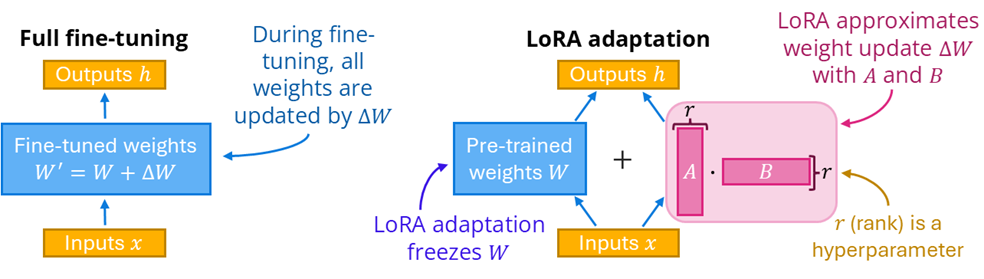
\includegraphics[width=0.76\textwidth]{figures/lora.png}
	\centering
	\caption{LoRA adapters are added in the attention layers to the query and valuey weight matrices \cite{Hu2021lora}.}

	\label{fig:lora}
\end{figure}

%===============================================================
\subsection{Related Work in Generative Design}
%===============================================================

The field of neural CAD generation has grown rapidly in recent years. Multiple approaches have been explored:

\begin{itemize}
	\item \textbf{CAD Agents}: Copilot the CAD software with a human in the loop
	\item \textbf{Graph Neural Networks}: Capturing the topological structure of CAD models through graphs
	\item \textbf{Transformer-based Methods}: Leveraging attention mechanisms for long-range dependencies
	\item \textbf{Multi-modal Learning}: Combining text, images, and geometry for conditional generation
\end{itemize}

The integration of LoRA with pre-trained generative models enables efficient adaptation to specialized domains without requiring large labeled datasets or extensive computational resources. This is particularly valuable for downstream applications where domain-specific data is limited.
